\subsection{Reference resolution}
\subsubsection*{Setup}
In the final experiments, the agents are tasked to produced and understand referring expressions only based on the implicit human knowledge present in the scenes, as for example the attributes of the objects.
Opposed to the previous experiments, explicit human language information as human referring expressions or one-hot encoded attributes are avoided.
By this, the agents can't just reuse these human referring expressions, but need to learn to generate them themselves during the language games just based on the visual input.
This is done similarly to the single model reference resolution task, described in Section \ref{sec:reference_resolution}.
As before, the sender has the same architecture as in the previous language games, encoding the bounding boxes of all objects.

The receiver is tasked to solve two tasks.
First, in the \textbf{coordinate reference resolver}, the agents are tasked to predict the center coordinates of the target object (see Figure \ref{fig:coordinate_predictor_game_architecture}).
The receiver is the same in both setups and is based on the \emph{reference resolver} + referring expressions, described in Section \ref{sec:reference_resolution}.
Again, instead of the included LSTM, the receiver uses the \emph{EGG} LSTM with the hidden size $h_r=500$ and $e_r=100$ to encode the message.
The dimensions of the coordinate predictor are fixed to $c=2048$, based on the previous results.
% SD: Just thinking: would there be a more systematic way to compare all the models? Perhaps if you write the parameters in a table or a text that is parallel. Then you could simply say, modal A + these changes. It would be much clearer to the reader how all models are rerlated and it would be easier for the reader to follow.
% DK: TODO
The euclidean distance between the resulting prediction of the center point and the true center of the target object is calculated and the weights of both agents are adapted accordingly.

\begin{figure}[ht]
    \centering
    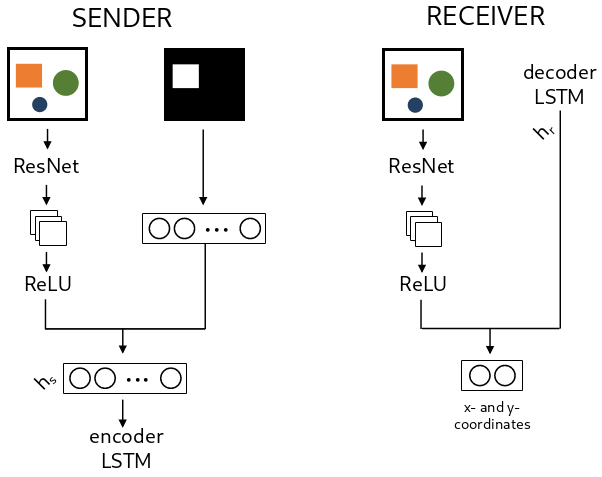
\includegraphics[width=.7\linewidth]{figures/arch_coordinate_predictor_game.png}
    \caption{Simplified architecture of the coordinate predictor game}
    \label{fig:coordinate_predictor_game_architecture}
    % SD: Again, why LSTM, are we inceremtally identifying the image while we are processing each input word?
    % DK: because it's a message sequence of discrete symbols (done)
\end{figure}

Secondly, in the \textbf{attention reference resolver}, the agents learn to point towards regions in the image, which is based on the \emph{attention reference resolver} described in section \ref{sec:reference_resolution}.
As before, the LSTM is replaced with the \emph{EGG} LSTM to parse the sender's message with the hidden size $h_r=500$ and $e_r=100$.
The dot product is calculated between each encoded region of the image and the encoded message, and the $softmax$ function is applied subsequently.
Figure \ref{fig:attention_predictor_game_architecture} shows the architecture.
The loss is calculated using \emph{binary cross entropy} between the predictions and ground truth regions.

\begin{figure}[ht]
    \centering
    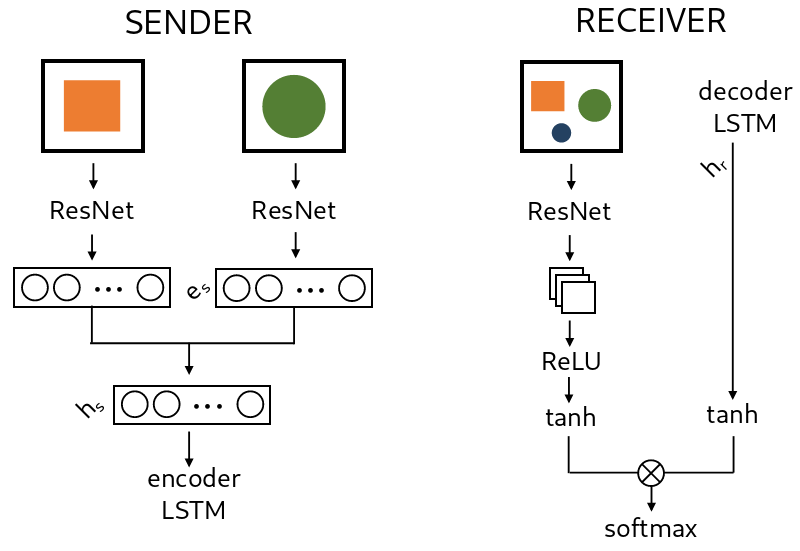
\includegraphics[width=.7\linewidth]{figures/arch_attention_predictor_game.png}
    \caption{Simplified architecture of the attention predictor game}
    \label{fig:attention_predictor_game_architecture}
    % SD: Again, why LSTM, are we inceremtally identifying the image while we are processing each input word?
    % DK: because it's a message sequence of discrete symbols (done)
\end{figure}

The experiments are conducted with the following hyperparameters: a learning rate of $2\times10^{-4}$, a temperature for the Gumbel-Softmax relaxation of 1 and \emph{Adam} \citep{Kingma2015} as optimizer.
The following values for the variables are compared:
\begin{itemize}
    \item $|V|$: 2, 10, 16, 50, 100
    \item $n$: 1, 2, 3, 4,  6
\end{itemize}

As in section \ref{sec:reference_resolution}, the agents are trained on the 'Dale-2', 'Dale-5' and 'CLEVR color' datasets to test if the agents are able to first communicate a target object and second describe the target object discriminatively with a small vocabulary.
The same metrics are used to evaluate the results as described in \ref{sec:reference_resolution}.

\subsection*{Results}
\begin{figure}[ht!]
    \centering
    \subfigure['Dale-2' dataset]{
        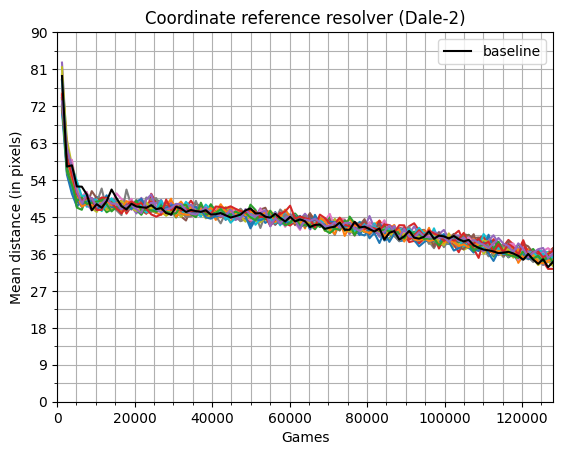
\includegraphics[width=0.485\linewidth]{figures/learning-curve_coordinate-predictor_dale-2.png}
        \label{fig:learning-curve_coordinate-predictor_dale-2}
    }
    \subfigure['Dale-5' dataset]{
        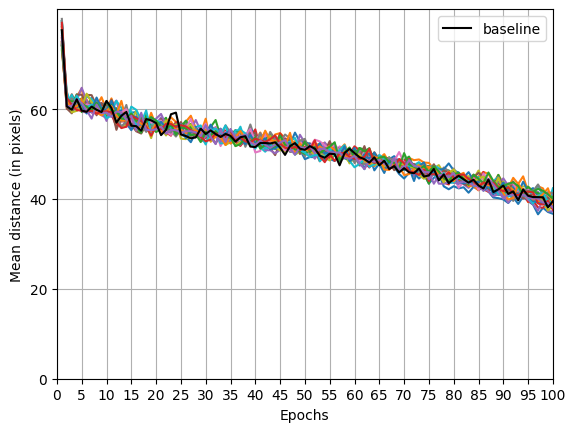
\includegraphics[width=0.485\linewidth]{figures/learning-curve_coordinate-predictor_dale-5.png}
        \label{fig:learning-curve_coordinate-predictor_dale-5}
    }
    \subfigure['CLEVR color' dataset]{
        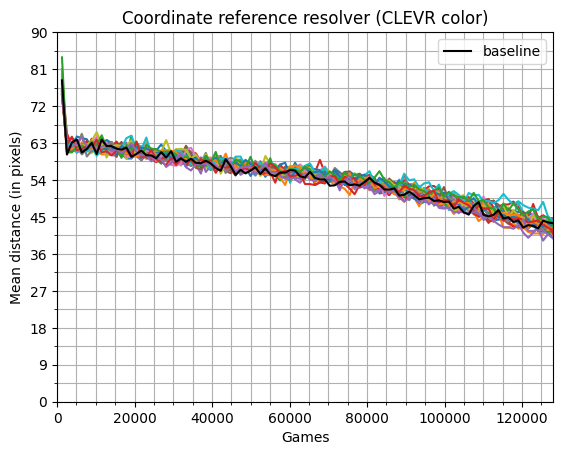
\includegraphics[width=0.485\linewidth]{figures/learning-curve_coordinate-predictor_colour.png}
        \label{fig:learning-curve_coordinate-predictor_colour}
    }
    \caption{Learning curves of all coordinate reference resolving games on each dataset. As almost no games beat the baseline, $|V|$ and $n$ are not highlighted separately. The baseline is marked in black.}
    \label{fig:learning-curves_coordinate-predictor}
\end{figure}

\begin{table}[ht]
    \centering
    \begin{tabular}{cc|cc|cc|cc}
        \toprule
                                      &         & \multicolumn{2}{c}{\textbf{Dale-2}} & \multicolumn{2}{c}{\textbf{Dale-5}} & \multicolumn{2}{c}{\textbf{CLEVR color}}                                                                                         \\  \cmidrule(lr){3-4}\cmidrule(lr){5-6}\cmidrule(lr){7-8}
        $n$                           & $|V|$   & \textbf{loss}                       & \textbf{Acc.}                       & \textbf{loss}                            & \textbf{Acc.}               & \textbf{loss}             & \textbf{Acc.}               \\\midrule
        \multicolumn{2}{c|}{baseline} & {34,49} & {34,3\%}                            & {38,13}                             & {30,31\%}                                & {42,72}                     & {18,28\%}                                               \\\midrule
        {1}                           & {2}     & \textcolor{purple}{34,91}           & \textcolor{purple}{34,81\%}         & \textcolor{purple}{40,61}                & \textcolor{purple}{25,48\%} & {39,13}                   & {25\%}                      \\
        {1}                           & {10}    & \textcolor{purple}{35,31}           & {40,15\%}                           & \textcolor{purple}{38,73}                & \textcolor{purple}{28,12\%} & \textcolor{purple}{44,19} & {20,53\%}                   \\
        {1}                           & {16}    & \textcolor{purple}{35,4}            & {42,93\%}                           & \textcolor{purple}{39,58}                & \textcolor{purple}{26,17\%} & {39,64}                   & {24,18\%}                   \\
        {1}                           & {50}    & {32,64}                             & {42,01\%}                           & \textcolor{purple}{38,99}                & \textcolor{purple}{28,52\%} & \textcolor{purple}{42,61} & {20,79\%}                   \\
        {1}                           & {100}   & \textcolor{purple}{36,73}           & \textcolor{purple}{31,21\%}         & \textcolor{purple}{40,25}                & \textcolor{purple}{24,91\%} & \textcolor{purple}{41,5}  & {21,44\%}                   \\
        {2}                           & {2}     & \textcolor{purple}{33,76}           & {40,67\%}                           & {35,86}                                  & {31,73\%}                   & \textcolor{purple}{41,79} & {22,14\%}                   \\
        {2}                           & {10}    & {31,37}                             & {43,27\%}                           & {37,23}                                  & \textcolor{purple}{30,34\%} & \textcolor{purple}{42,53} & \textcolor{purple}{19,75\%} \\
        {2}                           & {16}    & {31,19}                             & {46,27\%}                           & \textcolor{purple}{39,38}                & \textcolor{purple}{28,21\%} & \textcolor{purple}{41,74} & {22,7\%}                    \\
        {2}                           & {50}    & \textcolor{purple}{33,66}           & {39,28\%}                           & \textcolor{purple}{39,62}                & \textcolor{purple}{25,35\%} & \textcolor{purple}{45,63} & \textcolor{purple}{17,93\%} \\
        {2}                           & {100}   & \textcolor{purple}{35,1}            & \textcolor{purple}{34,81\%}         & \textcolor{purple}{39,86}                & \textcolor{purple}{27,3\%}  & \textcolor{purple}{45,45} & \textcolor{purple}{19,05\%} \\
        {3}                           & {2}     & {32,99}                             & {41,15\%}                           & {37,76}                                  & \textcolor{purple}{30,99\%} & \textcolor{purple}{46,45} & {20,92\%}                   \\
        {3}                           & {10}    & \textcolor{purple}{33,74}           & {38,89\%}                           & \textcolor{purple}{40,71}                & \textcolor{purple}{26,48\%} & \textcolor{purple}{44,53} & \textcolor{purple}{19,01\%} \\
        {3}                           & {16}    & \textcolor{purple}{34,18}           & {38,98\%}                           & \textcolor{purple}{38,52}                & \textcolor{purple}{30,03\%} & \textcolor{purple}{41,22} & {21,53\%}                   \\
        {3}                           & {50}    & \textcolor{purple}{34,38}           & {38,93\%}                           & \textcolor{purple}{39,52}                & \textcolor{purple}{26,74\%} & {38,4}                    & {24,87\%}                   \\
        {3}                           & {100}   & \textcolor{purple}{33,16}           & {40,19\%}                           & \textcolor{purple}{39,75}                & \textcolor{purple}{27,78\%} & \textcolor{purple}{41,29} & {21,83\%}                   \\
        {4}                           & {2}     & \textcolor{purple}{33,48}           & {40,36\%}                           & \textcolor{purple}{38,28}                & \textcolor{purple}{30,9\%}  & \textcolor{purple}{42,53} & {22,4\%}                    \\
        {4}                           & {10}    & \textcolor{purple}{35,01}           & {39,97\%}                           & \textcolor{purple}{40,88}                & \textcolor{purple}{26,39\%} & \textcolor{purple}{42,33} & {20,44\%}                   \\
        {4}                           & {16}    & \textcolor{purple}{35,59}           & \textcolor{purple}{35,59\%}         & \textcolor{purple}{37,91}                & {31,86\%}                   & \textcolor{purple}{41,9}  & {20,27\%}                   \\
        {4}                           & {50}    & \textcolor{purple}{34,99}           & {36,68\%}                           & \textcolor{purple}{40,89}                & \textcolor{purple}{23,26\%} & \textcolor{purple}{43,77} & \textcolor{purple}{18,36\%} \\
        {4}                           & {100}   & \textcolor{purple}{35,46}           & {37,46\%}                           & \textcolor{purple}{38,53}                & \textcolor{purple}{29,08\%} & {40,6}                    & {21,22\%}                   \\
        {6}                           & {2}     & \textcolor{purple}{34,97}           & {37,28\%}                           & \textcolor{purple}{39,52}                & \textcolor{purple}{29,69\%} & {40,53}                   & {24,7\%}                    \\
        {6}                           & {10}    & {32,39}                             & {43,53\%}                           & \textcolor{purple}{38,61}                & \textcolor{purple}{28,26\%} & {40,84}                   & {21,74\%}                   \\
        {6}                           & {16}    & \textcolor{purple}{34,87}           & \textcolor{purple}{34,38\%}         & \textcolor{purple}{39,03}                & \textcolor{purple}{26,82\%} & {40,34}                   & {23,31\%}                   \\
        {6}                           & {50}    & \textcolor{purple}{33,85}           & {37,07\%}                           & \textcolor{purple}{39,39}                & \textcolor{purple}{27,17\%} & {40,8}                    & {22,09\%}                   \\
        {6}                           & {100}   & \textcolor{purple}{34,62}           & {40,02\%}                           & \textcolor{purple}{39,46}                & \textcolor{purple}{25,48\%} & \textcolor{purple}{42,53} & \textcolor{purple}{18,4\%}  \\
        \bottomrule
    \end{tabular}
    \caption{Mean distance (loss) in pixels and accuracy in \% of the coordinate reference resolver after 128.000 games: $n$ are different maximum message lengths and $|V|$ are different vocabulary sizes.}
    \label{tab:results:coordinate-reference-resolver-game}
\end{table}

Figure \ref{fig:learning-curves_coordinate-predictor} show the learning curves for the \textbf{coordinate reference resolver}.
As visible, all configurations perform exactly as the baselines across all datasets.
The baselines show the predictions of the receiver without information of the sender, and correspond to the structural bias in the dataset.
This shows, that the agents don't communicate successfully in any of the configurations to solve the task and predict correct coordinates.
Table \ref{tab:results:coordinate-reference-resolver-game} shows the final results after 128.000 games on different datasets.
When looking at how the agents fare with each dataset, not much general improvement can be seen.
Most of the configurations don't beat the baseline, independently of the shown dataset.
If they do, they can improve the mean distance of the predicted coordinates to the center of the target object only by 2 to 4 pixels.
In other words, the guesses are still not consistently precise on the target objects and the agents instead learn to point towards the center of the scene, as the single models in Section \ref{sec:referring_expression_generation}.
However, an influence on the accuracy can be identified.
The accuracy evaluates how many of the predictions are on the target object.
An increase in the accuracy with a stable mean distance corresponds shows a behavior where the agents make more correct predictions on the target objects, while the wrong predictions a further away from the target object.
As a conclusion, this can mean, that the agents' predictions, both correct and incorrect are more confident.
This seems to happen on the 'Dale-2' dataset.
The mean distance is not improved, but the accuracy reaches in some configurations up to 46,27\%.
This is an increase of around 13\% compared to the baseline.
While this value is still lower than a random guess between the objects in the scene, it shows, that some information is exchanged between the agents.
The meaning of the messages however doesn't seem to correspond to any attribute or object to consistently solve the task.

Looking at the results on the 'Dale-5' dataset, no improvements for the mean distance nor the accuracy can be seen when a sender is involved.
However, while the loss stays again constant, the accuracy drops lower in many configurations, up to 7\% points to an accuracy of 23,26\%.
Again, this is an indicator that messages are transferred and interpreted by the receiver.
The receiver seems to use this information to focus more on the objects.
Since there are more distractors present in the 'Dale-5' dataset, the receiver more likely chooses one of those, as again no discriminating information about the target object seems to be transferred.

Lastly, the similar pattern on the mean distance is also visible for the 'CLEVR color' dataset.
The accuracy of the baseline is already lower to begin, and a sender can lift this score in almost all configurations.
But as for the other datasets, the final accuracy is still low and reaches a maximum of only 25\%.
The greater number of distractors seems to raise the complexity of the task even more.

These numbers align with the results of the single model, discussed in Section \ref{sec:referring_expression_generation}.
Hereby, the single model was only able to predict correct coordinates for the 'Dale-2' dataset with one distractor.
The higher complexity for the agents that includes more layers in the model as well as the discrete bottleneck raises the bar of the task too high to be solved in this configuration.
The second setup in this section, the \textbf{attention reference resolver}, tries to reduce the complexity, by not predicting precise geometric locations, but instead attending to larger areas.
The learning curves are shown in Figure \ref{fig:learning-curves_attention-predictor}.

As expected, the task is solver better by the agents, and they communicate successfully across all datasets.
Compared to the experiments in the previous sections, the learning is still generally slower, and the configurations diverge from the baseline overall later.
However, when the agents start to learn to communicate, the probability is boosted instantly to a higher level, where it again learns at a slower speed parallel to the baseline.
On the 'Dale-2' dataset, the boost is around 40\% points.
Most of the learning takes place in the first 40.000 games, but there are also two configurations that increase the performance very late after 70.000 and 105.000 games respectively.
Hereby, agents tend to learn faster the smaller their vocabulary size is.
The same applies as well to the message length.
Using the 'Dale-5' dataset, the probability masses are boosted around 30\% points when the agents start to communicate successfully.
Compared to the 'Dale-2' dataset, fewer configurations start to converge, while most achieve performances close to the baseline.
The smaller number of learning curves makes the analysis more difficult, but the same trend about the vocabulary size and the message length is still visible.
Interestingly, only one configuration with $|V|=2$ beats the baseline, but behaves relatively unstable over the remaining training.
On the other hand no configuration with $|V|=100$ is successful.
This indicates that one symbol too few to encode all meaning, but too many symbols are too difficult to learn.
This hypothesis is amplified by the results on the 'CLEVR color' dataset.
Only two configurations beat the baseline, both with a medium-sized vocabulary size and message length.
In both cases, the learning takes place relatively late, after 15.000 and 30.000 games respectively.

\begin{figure}[ht!]
    \centering
    \subfigure['Dale-2' dataset with different $|V|$ highlighted]{
        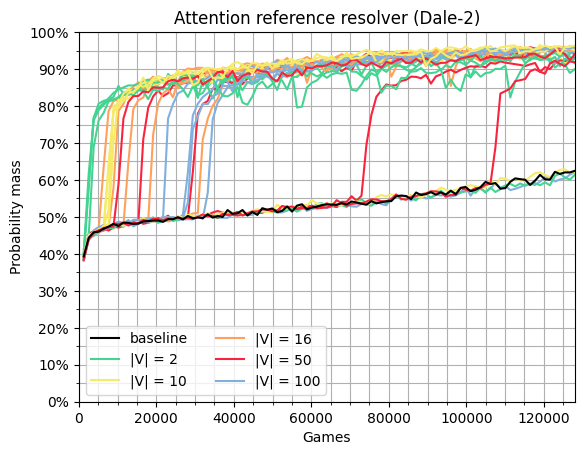
\includegraphics[width=0.485\linewidth]{figures/learning-curve_attention-predictor_dale-2_vocab-size.png}
        \label{fig:learning-curve_attention-predictor_dale-2_vocab-size}
    }
    \subfigure['Dale-2' dataset with different $n$ highlighted]{
        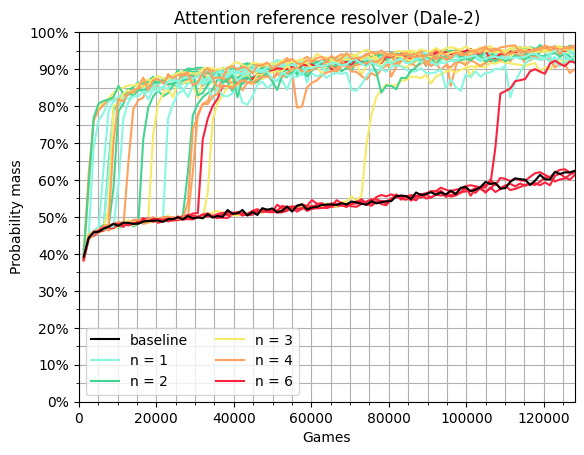
\includegraphics[width=0.485\linewidth]{figures/learning-curve_attention-predictor_dale-2_max-len.png}
        \label{fig:learning-curve_attention-predictor_dale-2_max-len}
    }
    \subfigure['Dale-5' dataset with different $|V|$ highlighted]{
        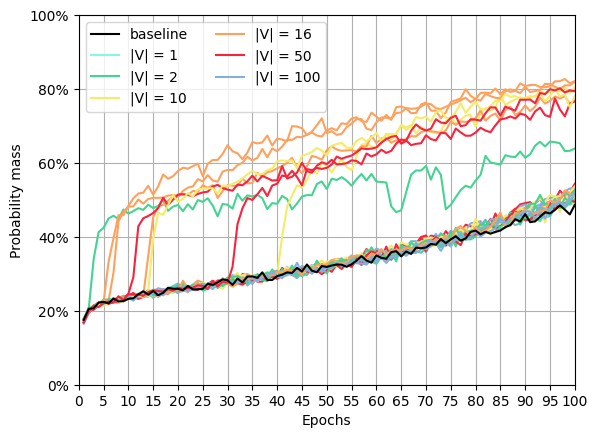
\includegraphics[width=0.485\linewidth]{figures/learning-curve_attention-predictor_dale-5_vocab-size.png}
        \label{fig:learning-curve_attention-predictor_dale-5_vocab-size}
    }
    \subfigure['Dale-5' dataset with different $n$ highlighted]{
        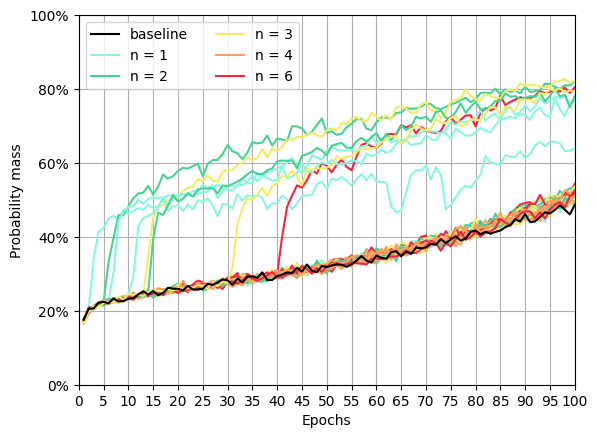
\includegraphics[width=0.485\linewidth]{figures/learning-curve_attention-predictor_dale-5_max-len.png}
        \label{fig:learning-curve_attention-predictor_dale-5_max-len}
    }
    \subfigure['CLEVR color' dataset with different $|V|$ highlighted]{
        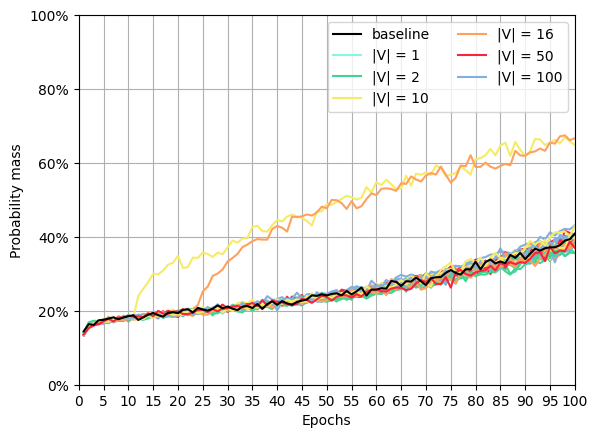
\includegraphics[width=0.485\linewidth]{figures/learning-curve_attention-predictor_colour_vocab-size.png}
        \label{fig:learning-curve_attention-predictor_colour_vocab-size}
    }
    \subfigure['CLEVR color' dataset with different $n$ highlighted]{
        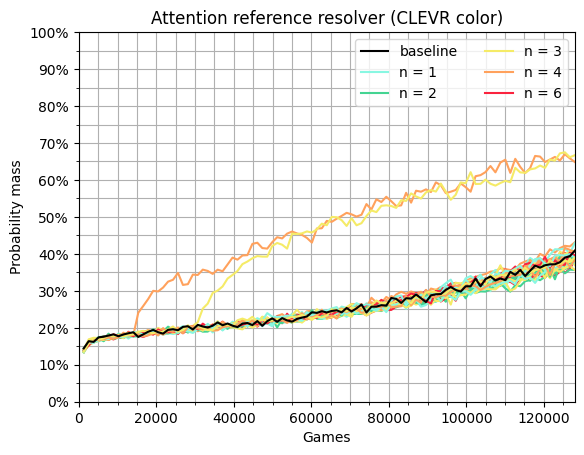
\includegraphics[width=0.485\linewidth]{figures/learning-curve_attention-predictor_colour_max-len.png}
        \label{fig:learning-curve_attention-predictor_colour_max-len}
    }
    \caption{Learning curves of all attention reference resolver games on each dataset. In the left column, the colors correspond to different vocabulary sizes $|V|$ while in the right column, the colors correspond to different message lengths $n$. The baseline is marked in black.}
    \label{fig:learning-curves_attention-predictor}
\end{figure}

\begin{table}[ht]
    \centering
    \begin{tabular}{cc|c|c|c}
        \toprule
                                      &           & \multicolumn{1}{c}{\textbf{Dale-2}} & \multicolumn{1}{c}{\textbf{Dale-5}} & \multicolumn{1}{c}{\textbf{CLEVR color}} \\  \cmidrule(lr){3-3}\cmidrule(lr){4-4}\cmidrule(lr){5-5}
        $n$                           & $|V|$     & \textbf{Probability mass}           & \textbf{Probability mass}           & \textbf{Probability mass}                \\\midrule
        \multicolumn{2}{c|}{baseline} & {62,16\%} & {49,61\%}                           & {41,68\%}                                                                      \\\midrule
        {1}                           & {2}       & {93,3\%}                            & {65,36\%}                           & \textcolor{purple}{39,22\%}              \\
        {1}                           & {10}      & {93,85\%}                           & \textcolor{purple}{46,97\%}         & \textcolor{purple}{40,1\%}               \\
        {1}                           & {16}      & {92,06\%}                           & {76,68\%}                           & \textcolor{purple}{36,43\%}              \\
        {1}                           & {50}      & {94\%}                              & {76,43\%}                           & \textcolor{purple}{39,97\%}              \\
        {1}                           & {100}     & {94,03\%}                           & \textcolor{purple}{54,14\%}         & \textcolor{purple}{40,27\%}              \\
        {2}                           & {2}       & {92,27\%}                           & \textcolor{purple}{52,15\%}         & \textcolor{purple}{33,64\%}              \\
        {2}                           & {10}      & \textbf{96,16\%}                    & {80,26\%}                           & \textcolor{purple}{36,53\%}              \\
        {2}                           & {16}      & {95,84\%}                           & \textbf{84,03\%}                    & \textcolor{purple}{39,65\%}              \\
        {2}                           & {50}      & {93,78\%}                           & \textcolor{purple}{52,24\%}         & \textcolor{purple}{39,56\%}              \\
        {2}                           & {100}     & {92,43\%}                           & \textcolor{purple}{53,23\%}         & \textcolor{purple}{37,68\%}              \\
        {3}                           & {2}       & {94,52\%}                           & \textcolor{purple}{51,97\%}         & \textcolor{purple}{37,09\%}              \\
        {3}                           & {10}      & {94,9\%}                            & \textcolor{purple}{53,47\%}         & \textcolor{purple}{38,24\%}              \\
        {3}                           & {16}      & {94,59\%}                           & \textbf{81,46\%}                    & \textbf{67,88\%}                         \\
        {3}                           & {50}      & {93,88\%}                           & {79,65\%}                           & \textcolor{purple}{40,36\%}              \\
        {3}                           & {100}     & {95,25\%}                           & \textcolor{purple}{48,52\%}         & \textcolor{purple}{42,55\%}              \\
        {4}                           & {2}       & {89,15\%}                           & \textcolor{purple}{51,98\%}         & \textcolor{purple}{39,68\%}              \\
        {4}                           & {10}      & \textbf{96,08\%}                    & \textcolor{purple}{48,03\%}         & \textbf{64,31\%}                         \\
        {4}                           & {16}      & {94,14\%}                           & \textcolor{purple}{49,81\%}         & \textcolor{purple}{40,84\%}              \\
        {4}                           & {50}      & \textbf{96,24\%}                    & \textcolor{purple}{48,79\%}         & \textcolor{purple}{43,61\%}              \\
        {4}                           & {100}     & {95,55\%}                           & \textcolor{purple}{49,65\%}         & \textcolor{purple}{42,85\%}              \\
        {6}                           & {2}       & \textcolor{purple}{59,68\%}         & \textcolor{purple}{53,57\%}         & \textcolor{purple}{38,43\%}              \\
        {6}                           & {10}      & \textcolor{purple}{63,46\%}         & \textbf{82,12\%}                    & \textcolor{purple}{40,11\%}              \\
        {6}                           & {16}      & {95,86\%}                           & \textcolor{purple}{50,71\%}         & \textcolor{purple}{40,61\%}              \\
        {6}                           & {50}      & {91,27\%}                           & \textcolor{purple}{52,55\%}         & \textcolor{purple}{40,21\%}              \\
        {6}                           & {100}     & \textcolor{purple}{60,27\%}         & \textcolor{purple}{46,92\%}         & \textcolor{purple}{41,98\%}              \\
        \bottomrule
    \end{tabular}
    \caption{Probability masses of the attention reference resolver after 128.000 games: $n$ are different maximum message lengths and $|V|$ are different vocabulary sizes.}
    \label{tab:results:attention-reference-resolver-game}
\end{table}

The final probability masses after 128.000 games are summed up in Table \ref{tab:results:attention-reference-resolver-game}.
Opposed to the \emph{coordinate reference resolver}, the baseline can already find and attend to the correct regions in many cases.
The probability mass, that is the sum of the predicted probabilities of all regions of the target object is higher than a uniform distribution (\approx 4,6\%) and a random guess of an object.
It reaches 62,16\% on the 'Dale-2' dataset, 49,61\% on the 'Dale-5' dataset and 41,68\% on the 'CLEVR color' dataset.
Interestingly, including a sender in the setup can improve the result for all dataset.
Looking at the 'Dale-2' dataset, almost all configurations beat the baseline and achieve performances of over 90\%, the best configurations reach even 96\%.
Only three configurations stay on the level of the baseline.
When comparing the results, mostly the message length $n$ seems to have an influence on the performance.
While configurations with $n=6$ can perform well, this is not constant.
All three configurations that don't pass the baseline are allowed to produce message with $n=6$.
$n \in \{3,4\}$ seem to help the agents the most to perform consistently well, but the difference to configurations with $n \in \{1,2\}$ is very small.
In both cases, the target object is unambiguously identified.
The small number of experiments doesn't allow definite conclusions on the influence of the vocabulary size $|V|$, though $|V|=2$ performs slightly worse than the remaining vocabulary sizes.
A correlation between $n$ and $|V|$ is not identifiable.

On the 'Dale-5' dataset, the agents already have bigger problems to beat the baseline.
Only 8 out of 30 configuration perform better and reach probability masses around 76\% to 84\%.
However, the increase compared to the baseline is with around 30\% points as high as on the 'Dale-2' dataset.
Smaller message lengths ($n \in \{1,2,3\}$) as well as a medium-sized vocabulary ($|V| \in \{10,16,50\}$) tend to help the agents more, to solve the task successfully.
As before, no correlation is visible with the few successful games.
That the agents struggle more with the 'Dale-5' dataset is not surprising.
First, the larger number of distractors makes it more difficult for the receiver to focus, as can be seen already in the baseline performances.
Additionally, in case the sender communicates the attributes of the target object to the receiver, more information needs to be encoded to uniquely describe the target object.
This is naturally more complex to learn for the agents.
Finally, since more objects are present, they are more likely clustered closer together, which can result in the identification of adjacent regions to the target regions.

The agents struggle the most on the 'CLEVR color' dataset.
Hereby, only two configurations perform better than the baseline and reach a probability mass of around 64\% to 67\%.
Both utilize a medium message length of $n \in \{3,4\}$ and a medium-sized vocabulary of $|V| \in \{10,16\}$.
Interestingly, several configurations with short message lengths of $n \in \{1,2\}$ perform worse than the baseline.
This indicates that there is communication between the agents, but it rather distracts the receiver from the target object towards the distractors.
The same argument for a more difficult task when more objects are involved can be made for the 'CLEVR color' dataset.
This dataset includes even up to 10 objects present in the scene which increases the likelihood that the receiver focuses on a wrong object.

\begin{figure}[ht]
    \centering
    \subfigure['Dale-2']{
        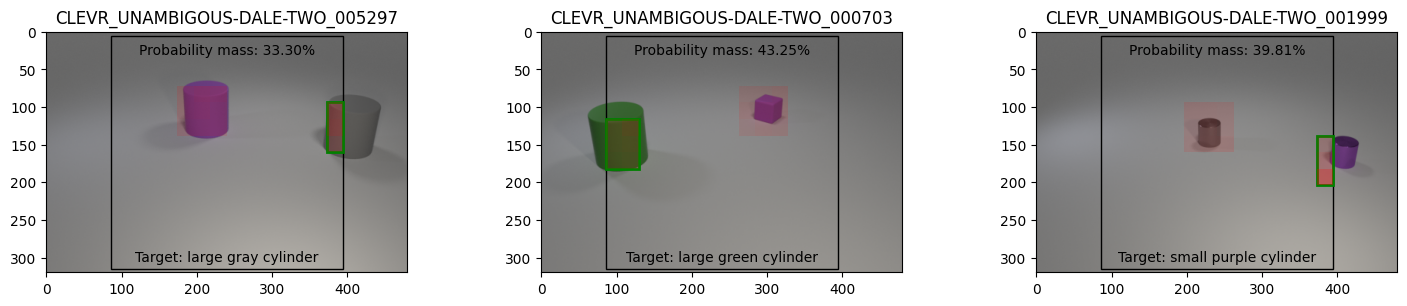
\includegraphics[width=.839\linewidth]{figures/visualization_games_dale-2_attention.png}
        \label{fig:visualizations_game_dale-2_attention}
    }
    \subfigure['Dale-5']{
        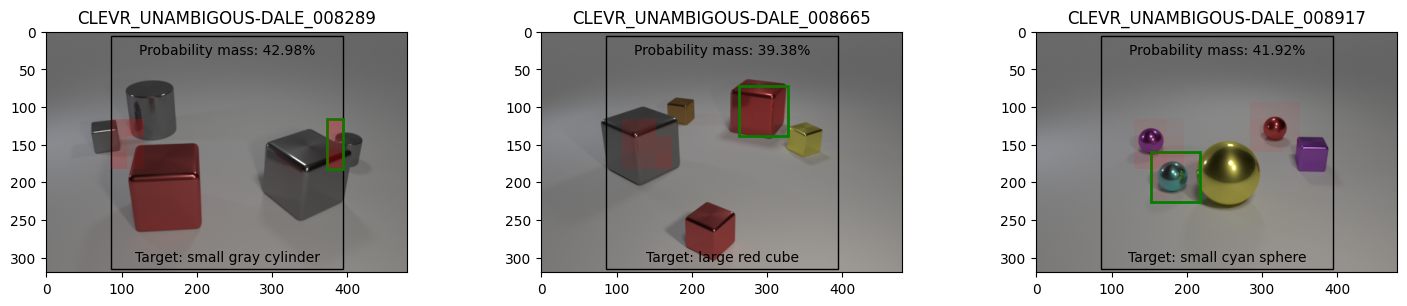
\includegraphics[width=.839\linewidth]{figures/visualization_games_dale-5_attention.png}
        \label{fig:visualizations_game_dale-5_attention}
    }
    \subfigure['CLEVR color']{
        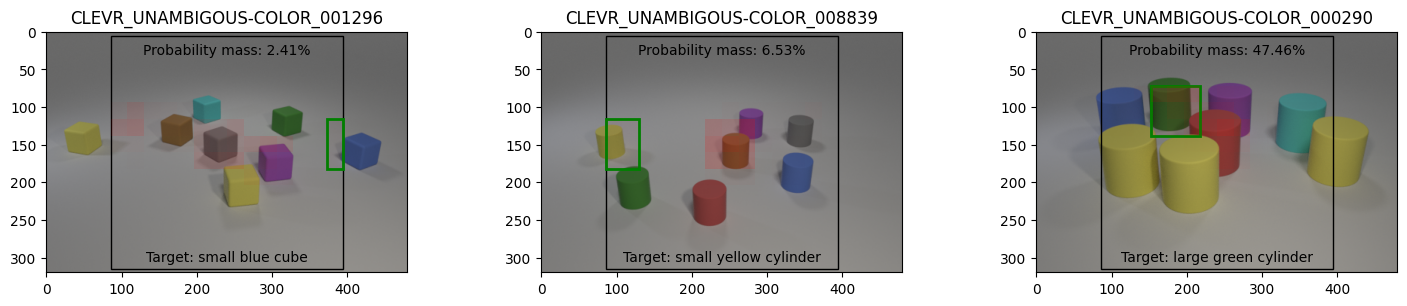
\includegraphics[width=.839\linewidth]{figures/visualization_games_colour_attention.png}
        \label{fig:visualizations_game_colour_attention}
    }
    \caption{Examples of the \emph{attention reference resolvers'} predictions in games with successful communication with a probability mass lower than 50\% on the 'Dale' and 'CLEVR color' datasets. The black rectangle shows the cropped section, the model is actually seeing after the image is preprocessed. The green rectangle surrounds the target region that needs to be predicted while the red regions show the actual predictions of the model. The more intense the red, the higher is the probability that the model assigned to this region.}
    \label{fig:visualizations_game_attention}
\end{figure}

Figure \ref{fig:visualizations_game_attention} shows examples of the wrongly identified regions on each dataset.
These are predictions by configurations in which the agents were successfully communicating.
In other words the sender was not able to transfer information to the receiver, even though a language had already emerged.
As can be seen on the 'Dale-2' dataset in Figure \ref{fig:visualizations_game_dale-2_attention}, similar problems about non-visible objects occur as for the single models described in Section \ref{sec:reference_resolution}.
These are in fact the main errors on this dataset.
However, in several cases (as in the central image), all objects are visible, and the agents still don't attend solely on the target object.
Rather than choosing one of the distractors, the agents usually attend to both objects relatively equally.
This indicates that the receiver is uncertain which object the sender is describing.
Similar errors also occur on both remaining datasets.
In contrast, the share of errors of the latter type is drastically higher.
Looking at the results on the 'Dale-5' dataset (see Figure \ref{fig:visualizations_game_dale-5_attention}), the model focusses usually on several objects at once.
While a general pattern is difficult to identify, the receiver tends to confuse the target object with distractors that share multiple attributes with each other.
In the central and right image, the wrongly identified distractors share both \emph{size} and \emph{shape} with the target object.
Finally, on the 'CLEVR color' dataset, no overall reason for the errors can be identified in the qualitative analysis.



% SD: This identifies that the problem lies in how the sender encodes the messages; what is its policy to generate longer strings or reuse the word. Without a policy the sender will never be motivated to encode longer messages and therefore rely on single-word expressions.
% SD: The second problem is the size of these networks. We should also test smaller embedding sizes than 10. Practice shows that the embedding sizes can be even several magnitues smaller than the vocabulary sizes, cf. the Bengio paper and word2vec.
% SD: The reason why the system is not performing well on the pointing task is that it does not have the right features to learn from. It ahs visual information WHAT these objects are (what do they look like) but they do not have information WHERE these objects are,. John Kelleher and I wrote an opiiuon piece about the lack of spatial knowledge required to model spatial descriptions in CNNs. The same problem is probably occuring here. Replacing the features or adding geometric features that would communicate geometric relations that allow pointing would improve the task and also we would expect that a vocabulary would emerge such that some words are more biased towards visual features (to identify objects) and some more to geometric features (to locate them), hence WHAT and WHERE.
% SD: J. D. Kelleher and S. Dobnik. What is not where: the challenge of integrating spatial representations into deep learning architectures. In S. Dobnik and S. Lappin, editors, Proceedings of the Conference on Logic and Machine Learning in Natural Language (LaML 2017), Gothenburg, 12 –13 June, volume 1 of CLASP Papers in Computational Linguistics, pages 41–52, Gothenburg, Sweden, November 2017. Department of Philosophy, Linguistics and Theory of Science (FLOV), University of Gothenburg, CLASP, Centre for Language and Studies in Probability.https://gup.ub.gu.se/publication/262970?lang=en
% SD: Overall, the thesis has a lot of potential if we could implement all this
% DK: TODO
